\documentclass{article}
\usepackage{amssymb,amsmath}
\usepackage{ifxetex,ifluatex}
\ifxetex
  \usepackage{fontspec,xltxtra,xunicode}
  \defaultfontfeatures{Mapping=tex-text,Scale=MatchLowercase}
\else
  \ifluatex
    \usepackage{fontspec}
    \defaultfontfeatures{Mapping=tex-text,Scale=MatchLowercase}
  \else
    \usepackage[utf8]{inputenc}
  \fi
\fi
\usepackage{ctable}
\usepackage{float} % provides the H option for float placement
\usepackage{graphicx}
% We will generate all images so they have a width \maxwidth. This means
% that they will get their normal width if they fit onto the page, but
% are scaled down if they would overflow the margins.
\makeatletter
\def\maxwidth{\ifdim\Gin@nat@width>\linewidth\linewidth
\else\Gin@nat@width\fi}
\makeatother
\let\Oldincludegraphics\includegraphics
\renewcommand{\includegraphics}[1]{\Oldincludegraphics[width=\maxwidth]{#1}}
\ifxetex
  \usepackage[setpagesize=false, % page size defined by xetex
              unicode=false, % unicode breaks when used with xetex
              xetex]{hyperref}
\else
  \usepackage[unicode=true]{hyperref}
\fi
\hypersetup{breaklinks=true, pdfborder={0 0 0}}
\setlength{\parindent}{0pt}
\setlength{\parskip}{6pt plus 2pt minus 1pt}
\setlength{\emergencystretch}{3em}  % prevent overfull lines
\setcounter{secnumdepth}{0}

\title{Descriptives}
\author{Rapport package team @ https://github.com/aL3xa/rapport}
\date{2011--04--26 20:25 CET}

\begin{document}
\maketitle

\subsection{Description}

This template will return descriptive statistics of a numerical, or a
frequency table of a categorical variable.

\subsubsection{Variable description}

The dataset has 709 observations with 709 valid values (missing: 0) in
``it.edu'' (``Internet usage for educational purposes (hours per
day)''). This variable seems to be numeric.

\subsubsection{Base statistics}

\ctable[pos = H, center, botcap]{lllllllllllllllllllll}
{% notes
}
{% rows
\FL
 & \textbf{0} & \textbf{0.5} & \textbf{1} & \textbf{1.5} & \textbf{2} & \textbf{2.5} & \textbf{3} & \textbf{3.5} & \textbf{4} & \textbf{4.5} & \textbf{5} & \textbf{5.5} & \textbf{6} & \textbf{6.5} & \textbf{7} & \textbf{8} & \textbf{8.5} & \textbf{9} & \textbf{10} & \textbf{12}
\ML
1 & 61.00000 & 102.00000 & 204.00000 & 27.00000 & 109.00000 & 17.00000 & 66.00000 & 2.00000 & 37.00000 & 2.00000 & 33.00000 & 1.00000 & 13.00000 & 1.00000 & 1.00000 & 25.00000 & 1.00000 & 2.00000 & 2.00000 & 3.00000
\LL
}

\subsubsection{Histogram}

\begin{figure}[htbp]
\centering
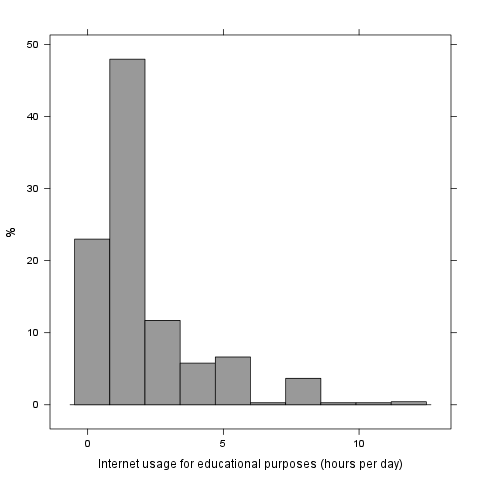
\includegraphics{598faf698f82b8217e0ed3137a62daaf.png}
\caption{}
\end{figure}

It seems that the highest value is 12 which is exactly Inf times higher
than the smalles values (0).

If we suppose that "Internet usage for educational purposes (hours per
day) is not near to a normal distribution (test: , skewness: 1.8593,
kurtosis: 6.8501), checking the median (1) might be a better option
instead of the mean. The interquartile range (2) measures the statistics
dispersion of the variable (similar to standard deviation) based on
median.

\end{document}
